\documentclass[conference]{IEEEtran}
\IEEEoverridecommandlockouts
% The preceding line is only needed to identify funding in the first footnote. If that is unneeded, please comment it out.
\usepackage{cite}
\usepackage{amsmath,amssymb,amsfonts}
\usepackage{algorithmic}
\usepackage{graphicx}
\usepackage{textcomp}
\def\BibTeX{{\rm B\kern-.05em{\sc i\kern-.025em b}\kern-.08em
    T\kern-.1667em\lower.7ex\hbox{E}\kern-.125emX}}
\begin{document}

\title{Automated Process Migration in LXC}

\author{\IEEEauthorblockN{Anamika Avinash}
\textit{Dublin City University}\\
Dublin, Ireland \\
anamika.avinash2@mail.dcu.ie
}

\maketitle

\begin{abstract}
Container technology is a method to execute multiple isolated sets of systems on a control host using a single kernel. This type of isolation facilitates the migration of the process between two containers. Linux Containers (LXC) are considered in this paper. Process migration mechanism can be employed under circumstances which requires the user to offload work from systems with high CPU utilization to idle systems. Using the Checkpoint/Restore In Userspace (CRIU) process migration tool, the intended process for migration is checkpointed and frozen into a set of files and transferred on to the destination system. Following this the CRIU tool rebuilds and executes the process from down-up based on the set of files that were transferred before. This paper assumes a hypothesis that process migration at the container-level is possible and can be automated. After instantiation with necessary experiments in varying scenarios, the paper disproves the hypothesis providing significant rationale.  

\end{abstract}

\begin{IEEEkeywords}
process migration, CRIU, LXC.
\end{IEEEkeywords}

\section{Introduction}
\label{sec: 1.introduction}
Load balancing, efficient resource utilization and increased performance are the vital features due to which process migration has been gaining increased popularity in the field of distributed systems. This procedure is generally done manually. Automating gives the functionality a positive edge in time consumption, consistency and robustness, to name a few, over the traditional manual method. This paper analyses process migration in Linux containers considering the checkpoint/restore method called CRIU.

\subsection{Containers}
\label{subsec: 1a.containers}
Containers employ lightweight operating system level virtualization consisting of a single kernel which permits the existence of multiple isolated user-space systems\cite{Dua2014VirtualizationPaaS}. The isolation provided by it is similar to the ones already in use in virtual machines but in addition to it, much better CPU performance is also a given boon. LXCs are Linux containers where the host system and the containers function on the same Linux kernel as shown in \ref{fig 1: Container}. One of the main advantages of Linux Containers over virtual machines (VM) is the reduced resource overhead. \cite{Dua2014VirtualizationPaaS}

\begin{figure}[h!]
%\vspace{-0.2cm}
 \centering
 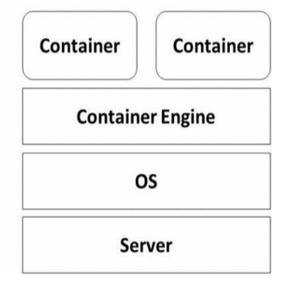
\includegraphics[width = 6cm]{Container.png}
 \caption{Container Architecture (Source:\cite{Ann2015PerformanceMachines})}
 \label{fig 1: Container}
\end{figure}


\subsection{Process Management} 
\label{subsec: 1b.process management}
Process is said to be a program or thread which is being executed in a computing context. Process management is considered to be essential in the functioning of an operating system. Its objective is to administer resources, isolate the processes, permit synchronization and allow them to exchange any form of messages or information they require. 

\subsection{Process Migration}
\label{subsec: 1d.process migration}
Process migration, as the name indicates, is the procedure to transfer a running process or processes between machines. It had its origin with the advent of distributed computing which is a specialized field that examines distributed systems which is a model where the components located on a geographically limited computers communicate by passing messages to achieve a goal. 
It has added advantages such as duplicating processes to increase reliability and stability, moving processes running on sensitive data to a secure instance to increase security and functionality and so on. Process migration finds application in migrating monolith applications to microservices as well \cite{OConnor2017ContinuousPerspective}. According to recent advances in this technology, there are multiple tools which are developed to achieve these goals. A good migration mechanism is based on how efficient it is in terms of time, redundancy, latency and cost. Lower the amount of dependencies, better it is for the user and it decreases the complexity of a software process.


\subsection{CRIU} 
\label{subsec: 1c.criu}
Checkpoint/Restore in user-space or CRIU is a software tool with pioneering implementation focusing on Higher Availability (HA) \cite{Li2015ComparingAvailability} features for containers which function on the Linux operating systems. High Availabilty is a feature which ensures the operational performance of a system which is agreed upon priorly. As shown in \ref{fig 1: CRIU}, CRIU enables a user to freeze an executing process or a part of it and transfer it as a conglomeration of files on disk\cite{Pickartz2016MigratingCRIU}. This tool also allows snapshots, remote bugging, network load balancing and many more scenarios.

\begin{figure}[h!]
%\vspace{-0.2cm}
 \centering
 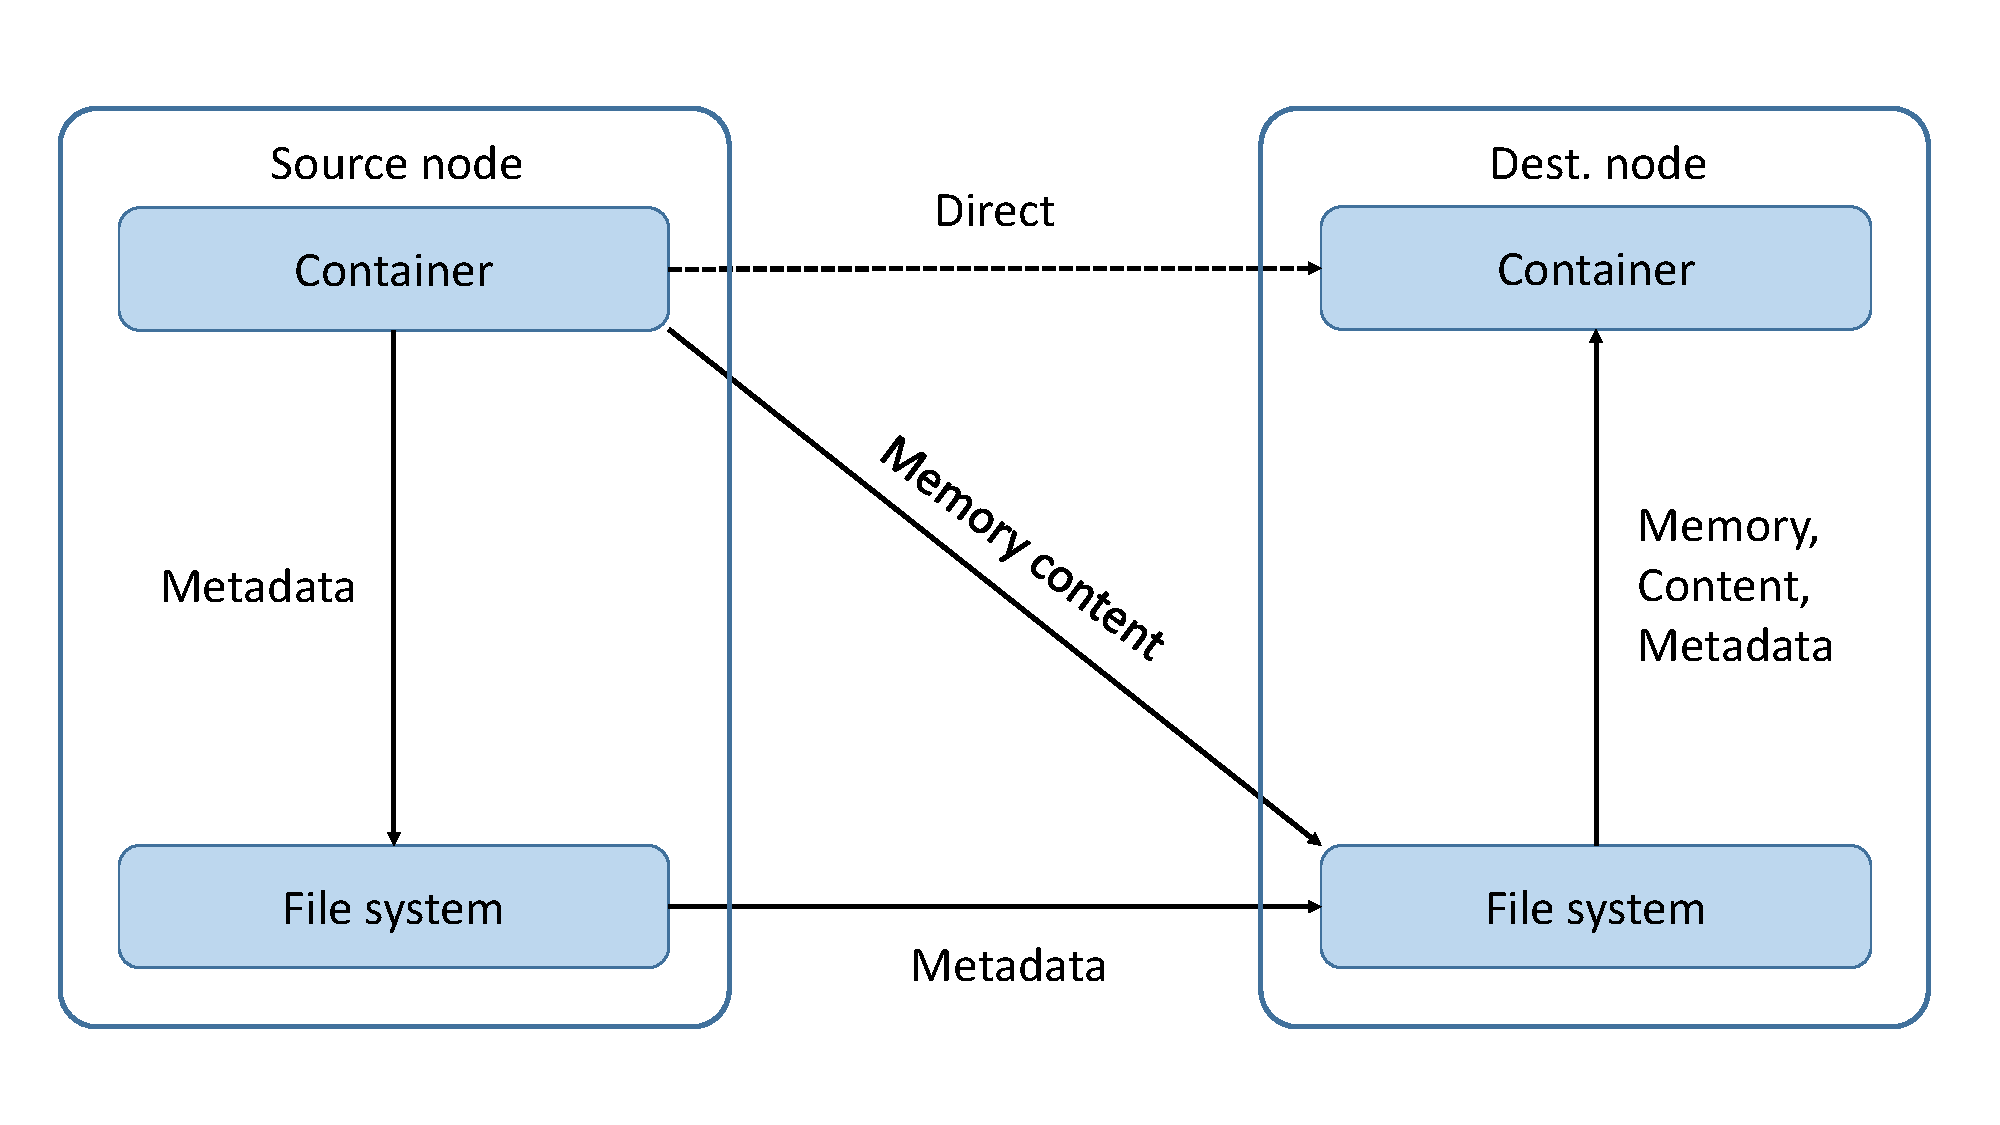
\includegraphics[width = 8cm]{CRIU.pdf}
 \caption{Checkpoint/Restore In Userspace. Source: \cite{Pickartz2016MigratingCRIU}}
 \label{fig 2: CRIU}
\end{figure}

This paper assumes a hypothesis that process migration at the container-level is possible and can be automated considering the successful adoption of process migration at the host-level. The remainder of the paper is structured as follows. Section \ref{sec: 2.Background} provides a background of the research on the related technologies. Section \ref{sec:3 Analysis Process Migration} describes the experiment conducted  for the analyses of process migration at container-level which includes \ref{subsec:3.1 CRIU in action} CRIU in action and \ref{subsec: 3b. Experimental Setup} Experimental Setup. Section \ref{sec: 4.Conclusion and Future Work} provides the conclusion and future work based on the experiments performed.  

\section{Background}
\label{sec: 2.Background}

A distributed computing system\cite{Salman2014TheSystems} is a set of computing nodes that are connected across a network. They merge to perform a large number of tasks. Generally, load balancing aims to utilize resources to their maximum potential. Main objective is to distribute the work across the network of nodes to reduce the mean task response duration and obtain higher efficiency. One of the important techniques considered in industry and academia to achieve significant improvement of load balancing measures is \emph{Process Migration}. 

%start with process migration
In 2000, Milojicic et al \cite{Milojicic2000ProcessMigration} summarized the important concepts and methodologies and provided an overview by surveying the field of process migration. This survey presents an outline on the details of process migration implementation based on case studies, misconceptions about the field and the actual drawbacks. The concepts include checkpointing and migration mechanism on Linux systems.

Gerofi et al \cite{Gerofi2010AnEnvironments} put forward a well planned process migration mechanism which comes handy when the process is handling a huge number of network connections. Additionally, an attempt to equalize loads on all the distributed machines was implemented through a decentralized middleware that factors process migration among the cluster nodes.

In 2014, Medina and Garcia \cite{Medina2014AMachines} surveyed mechanisms for migration in virtualized environments which are primarily classified into process migration, memory migration and suspend/resume migration. Multiple process migration mechanisms such as Zap\cite{Osman2002TheZap} and Autopod \cite{Potter2005AutoPod:Loss}  are discussed briefly in this paper.

Process migration technique for load balancing was discussed by Shah and Kapadia \cite{Shah2012LoadSystem} which focused on two algorithms namely, sender-initiated algorithm and the receiver-initiated algorithm. Sender initiated algorithm is based on non-preemptive migration and the receiver initiated algorithm is based on preemptive migration. The paper outlines both the algorithms and then concludes that process migration can be used for efficient load balancing


In 2005, Jason Duell \cite{Duell2005TheBLCR} devised the design and implementation of Berkley Lab's Linux Checkpoint/Restart which tackles a missing feature in linux clusters namely checkpoint/restore implementation at the kernel level. Commonly this system is referred to as BLCR and can be utilized as a standalone system for applications or parallel communication or a job scheduling system. 


Pickartz et al \cite{Pickartz2016MigratingCRIU} enabled migration of Linux Containers (LXC) through the implementation of a libvirt driver. Checkpoint Restore In Userspace mechanism is leveraged for the lxctools driver to support migration. CRIU saves sets of files which contains the state of the process by forming checkpoints. Following which, CRIU accesses /proc file system to retrieve information such as process ID (PID), file descriptors threads and so on. The collection of the memory and credentials is also done. After the process of checkpointing, the process can continue executing or may be terminated. In restoration process, the CRIU with the assistance of timers, credentials, threads etc, rebuilds the process tree and reads the image files. After this, the memory is rebuilt and the execution of the process can continue. 

In all the papers discussed above, the checkpoint restore functionality of process migration is widely adopted and discussed at the host-level. To tackle load balancing, migrating huge applications to microservices running on a container, process migration may be applied. In this paper, an hypothesis assuming that process migration can successfully be implemented on the container-level and can be automated. Thorough and experimental analyses at the container level in different scenarios is done and the findings are presented in a simplified way. 

\section{Analysis of Process Migration in Containers}
\label{sec:3 Analysis Process Migration} 
This section analyses process migration, the various prerequisites required, the procedure followed, obstacles encountered and attempts employed to overcome them. 

\subsection{CRIU in Action}
\label{subsec:3.1 CRIU in action}
The latest version of CRIU is 3.3 "Crystal Pelican". CRIU is a migration utility tool and is shown in a simple manner in \ref{fig 2: CRIU}. Using CRIU enables the user to migrate an executing application from the source system to the destination system. This is achieved by the following steps. On running the CRIU's checkpoint command the process running is frozen following which the image files are created. 

Image files are referred to the files which contain the state of the process. These image files can be in one of the three formats, namely the google protocol buffer format (protobuf), images which consist of binary data and a third part format (raw images). All of these files commence with 2 32-bit magic cookies in which the first cookie describes the type of file it is and the second cookie is optional sub-type of the image, if any.  Additionally, the images can be of three types as well. The first type is called inventory file which describes the set only and does not have any sub-type magic associated with it. The second type is called Auxiliary file. This type of image is not an image but the criu utility tool produces an image in the protobuf format. The third type is a regular image file.  For this demo, the format of the image chosen is the google protocol buffer format and a regular image file. At this point there are two ways that the migration can take place.

In the first method, the process which is frozen can be made to stop executing at the moment when it is checkpointed which can be a disadvantage as the execution is terminated until the process is rebuilt at the destination. The image files can be stored in two ways depending upon the need and the access that is required to be granted. If the process is meant to be shared among more than the source and the destination, the image files of the process has been created can be stored on the shared drive on the source machine. This grants access to more than one system at a time. If the process is supposed to be shared between only two systems, the checkpointed image files can be copied directly to the intended system. As mentioned in the before paragraph, the images are stored on google protocol buffer format, hereon referred to as protobuf. These files reside in the protobuf/ directory on the system. The files consist of multiple files. To name  a few - \emph{inventory}, which is an array file and contains an overview description of images and is named as inventory.proto. \emph{eventpoll} files which is also an array file which contains information on the process pertaining to the target file such as file descriptors, basic information and so on. \emph{core} files are single-entry files which, as the name indicates, contains data on the core process such as sigmask, name etc and also the dependent information such as registers, stacks and so on. In addition to these files there are many more files that are created which provides information on various necessary attributes such as netdev, utsns, mountpoints, tcp-stream etc. In this method, the source system terminates the execution of the process as the very moment that it has been checkpointed and the image files are created. They are then dumped into files on the destination system or a shared drive as need be. 

In the second method, a slight change can make sure the disadvantage specified at the beginning of the description of the first method can be overcome. Using this way, whenever the process is checkpointed and image files are created, the executing process to be migrated is not terminated but continues to execute on the source system until the control is switched over to the destination system. 

During the migration of processes, the memory is mapped and dumped in mm.img images but these files have information only on the virtual memory areas. These dumps contains the information of individual pages and data on which address locations in the virtual memory should reside in. Dumps pertaining to memory are stored in two images, namely pagemap and pages. Pagemap, as the name indicates, contains mapping information of the data. Pages contain plain sets of full page data. The memory areas which are in use by the task, if any file is mapped to it and shared memory areas are determined using \verb|smap_files| and \verb|map_files| present inside the /proc directory which are associated using links. Vital flags reside in the pagemap file also under the \emph{/proc} directory. The indicator \emph{present} implies that the physical page and the ones that are not present are assumed not to be dumped yet. The pages from the task's system are converted into a pipe using Ptrace with vmsplice. 

Rebuilding the process from the dump files that are created during the checkpoint is called restoring. Prior to explaining the restoration process, the concept of Copy-On-Write (COW) and shared memory are worth taking a look at. Until the tasks get COW-ed, there is a possibility that the pages shared between tasks might be a part of an anonymous private mapping. To tackle this, CRIU pre-restores those pages prior to forking the child processes. For the creation of shared memory area, the creator is first determined. Currently, the \emph{memfd} system call is used which accomplishes \emph{mmap-s} the region but also works for various userspaces due to which the creator creates the memory file descriptor (memfd) and all the other get one through \emph{fd} file in the \emph{/proc/pid} directory link which when compared to the \verb|map_files|, is not that strict. Restoration of memory is done in multiple ways.

Restoring memory can be done by opening all the mm.img image files and reading the mappings in it. By doing this, the shared memory partition or segment can be resolved and simultaneously check if any special-care mapped files are present. This is the most commonly utilized method. Additionally there are a few more, namely - open file mapping, restore mappings in their places, open shared mappings etc.

Memory mapping is followed by CRIU's restorer context which happens to be the final stage of the rebuilding process. It is devoid of libraries and is Position Independent Executable(PIE) compiled and can function on limited amount of memory. In this stage, CRIU restores memory, timers, credentials and threads adhering to the destination systems environment.

\subsection{Experimental Setup}
\label{subsec: 3b. Experimental Setup}

\begin{figure}[h!]
\centering
 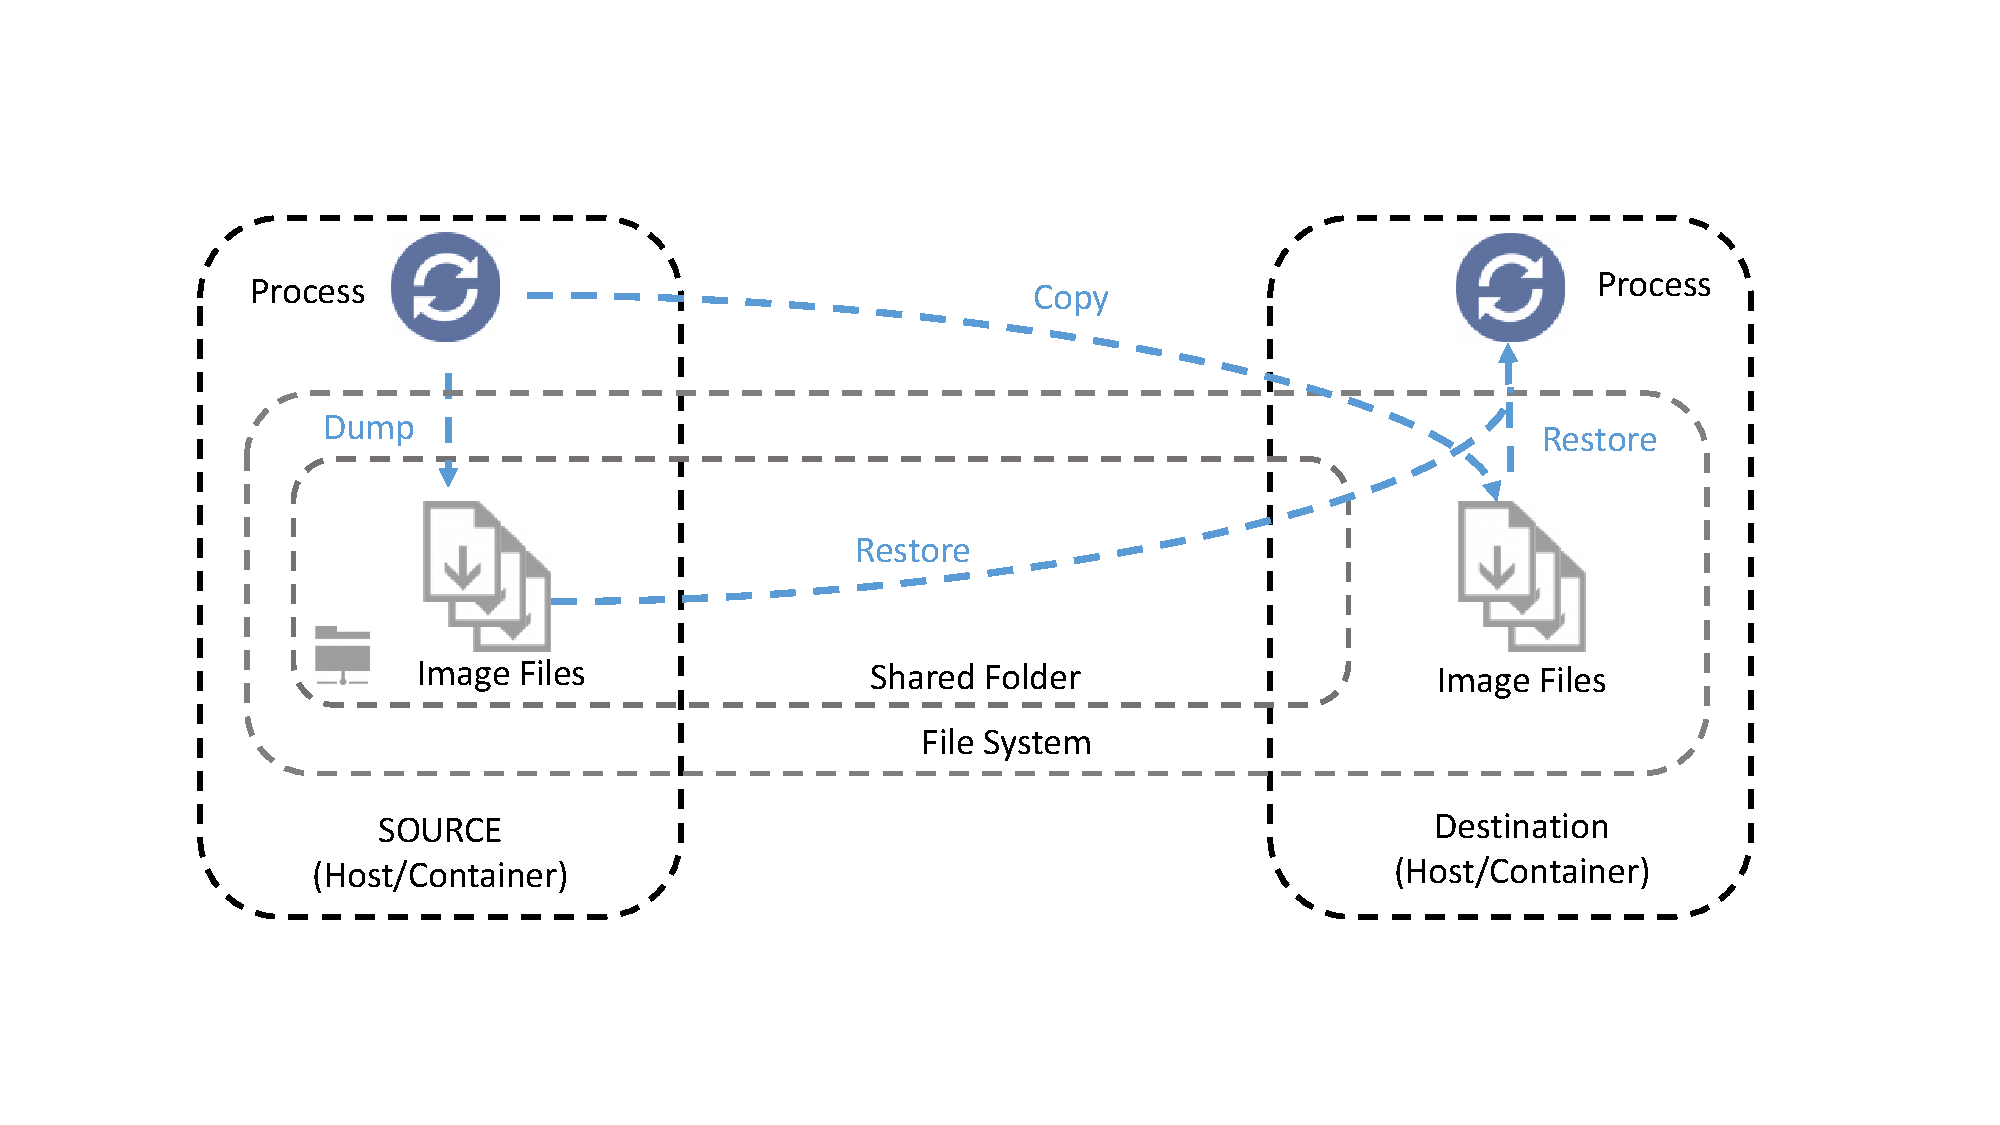
\includegraphics[width = 9.2cm]{Experiment.pdf}
 \caption{Experimental Setup Overview}
 \label{fig 1: CRIU}
\end{figure}

The host system used in this setup is running on Ubuntu 14.04.5 LTS kernel and so are the LXC containers. The Ubuntu 16.04.3 LTS kernel can also be used. The LXC containers run on the same kernel version as that of the host machine which in turn gives them an advantage of having almost zero overhead and additionally being very fast as well. The container imposes very little overhead when compared to a virtual machine \cite{Ann2015PerformanceMachines} because the operating system's interface is used to execute programs in virtual partitions unlike having to be executed on an intermediate virtual machine. Checkpoint/Restore In Userspace, CRIU, is installed on the host and the containers as well running on version 3.3 "Crystal Pelican".

\begin{table}[htbp]
\caption{Source/Destination Machine Combination}
\begin{center}
\begin{tabular}{|c|c|}
\hline
\textbf{Source}&\textbf{Destination} \\
\cline{1-2} 
\hline
Host & Host  \\
\hline
Container & Container  \\
\hline
Host & Container \\
\hline
Container & Host \\
\hline
\end{tabular}
\label{table 1}
\end{center}
\end{table}

Pre-requisites for the environment setup include:
\begin{itemize}
    \item \textbf{gcc, make, build-essential}: these libraries are needed as CRIU is written in C-language.
    \item \textbf{libprotobuf-dev libprotobuf-c0-dev protobuf-c-compiler protobuf-compiler python-protobuf}: these libraries are needed as CRIU uses google protocol buffers to read/write images.
    \item \textbf{libnl-3-dev libnet-dev}: network driver libraries.
\end{itemize}

To check if the installation of all the softwares were functioning, a script was executed which initiated a process in one of the systems, for the sake of simplicity lets refer to this as the source system and the system to which it is supposed to be migrated to as the destination system.

Lets consider the first scenario according to the table shown above. The source and the destination systems are both host machines and are running on Ubuntu 14.04 64-bit as as shown in Table \ref{table 2}. 

\begin{table}[htbp]
\caption{Scenario 1: Host-Host}
\begin{center}
\begin{tabular}{|c|c|}
\hline
\textbf{Source}&\textbf{Destination} \\
\cline{1-2} 
\hline
Host & Host  \\
Ubuntu 14.04 amd64 & Ubuntu 14.04 amd64 \\
\hline
\end{tabular}
\label{table 2}
\end{center}
\end{table}


In this scenario, a test script is created that executes a process in the source host system. Prior to this, CRIU utility tool is installed and configured according to the pre-requisites mentioned above. A check on the CRIU should indicate \emph{Looks good}, this is performed using the following command: \\

\noindent\verb|$sudo criu check| \\

The running process is dumped as image files [.img] with the following command: \\

\noindent\verb|$sudo criu dump -t $PID --images-dir| 
\verb|/path/to/folder --shell-job| \\

\noindent\verb|$PID| refers to the process ID of the running process, \verb|--images-dir| option can be used to specify where the image files should be dumped. \verb|--shell-job| option is required to dump processes running through a terminal. Similarly if a process has open TCP connections \verb|--tcp-established| option should be specified. Image files generated can be copied to the destination or the image dump folder can be made a shared folder between source and destination systems. The image files can be copied to the destination system using the following command:  \\

\noindent\verb|$sudo scp -r /path/to/source/folder|
\verb|user@destination_address:|
\verb|/path/to/destination/folder| \\

The copied images in the destination system can be used to restored as a process using the following CRIU command:\\

\noindent\verb|$sudo criu restore --images-dir| 
\verb|/path/to/folder --shell-job| \\

\noindent Since the process is restored in a different host, no need to specify \verb|$PID| in the restore command. The process was successfully migrated in this scenario. \\

In scenario 2, the process is attempted to migrate from Ubuntu 14.04 64-bit host to Linux Container LXC Ubuntu 14.04 64-bit as shown in Table \ref{table 3}. The step is to install the LXC on the host system. This is performed using the following commands:

\begin{verbatim}
$sudo add-apt-repository ppa:ubuntu-lxc
/daily
$sudo apt-get update
$sudo apt-get install lxc
\end{verbatim}

\begin{table}[htbp]
\caption{Scenario 2: Host-Container}
\begin{center}
\begin{tabular}{|c|c|}
\hline
\textbf{Source}&\textbf{Destination} \\
\cline{1-2} 
\hline
Host & Container  \\
Ubuntu 14.04 amd64 & LXC Ubuntu 14.04 amd64 \\
\hline
\end{tabular}
\label{table 3}
\end{center}
\end{table}

In this scenario, a test script is created that executes a process in the source host system. The process is dumped and the image files are copied to the destination container. The commands to dump the process and copy the image files are discussed in the previous scenario. 

CRIU is installed on the destination system, the CRIU installation failed as the container system could not access the procfs filesystem as this is mounted with read-only access. As a solution, the configuration of the LXC container was changed to re-mount the procfs with read-write access. The configuration file of the container is found at \verb|\var\lib\lxc\container_name\config|. The following two lines were added to the \verb|config| file:

\begin{verbatim}
lxc.mount.auto = proc sys cgroup

lxc.mount.auto = proc:rw sys:rw 
cgroup-full:rw
\end{verbatim}

\noindent CRIU restore resulted in an error as follows: 

\begin{verbatim}
Can't open -1/sys/kernel/ns_last_pid
on procfs: Permission denied
\end{verbatim} 

\noindent Though the container has read-write access to \verb|procfs|; \verb|criu check| returns \emph{Looks good.}, the system fails to access the proc file system. After thorough research on CRIU issues, it is found out processes cannot be rebuilt on containers and this is unresolved flagged issue in LXC development. \\

In scenario 3, process migration is attempted from container LXC Ubuntu 14.04 64-bit (source) to host Ubuntu 14.04 64-bit (destination). A demo process is created by running a small script which displays current time every second to the terminal. 

\begin{table}[htbp]
\caption{Scenario 3: Container-Host}
\begin{center}
\begin{tabular}{|c|c|}
\hline
\textbf{Source}&\textbf{Destination} \\
\cline{1-2} 
\hline
Container & Host  \\
LXC Ubuntu 14.04 amd64 & Ubuntu 14.04 amd64 \\
\hline
\end{tabular}
\label{table 4}
\end{center}
\end{table}

\noindent Similar to the previous scenarios, LXC is created on the host system and CRIU is installed on both host and container. When attempted to dump the process in the container, the following error was encountered:

\begin{verbatim}
Error (compel/src/lib/ptrace.c:27): 
suspending seccomp failed: 
Operation not permitted
\end{verbatim}

\noindent \emph{seccomp} is kernel security mechanism in Linux to filter system calls. CRIU to run in container requires seccomp to be suspended. Hence, fails to dump the process. A workaround to overcome this issue is yet to be developed in LXC. 

From scenario 2 and 3, it is observed that a process cannot be dumped or restored inside a container, it is safe to conclude that scenario 4 where a process is migrated from one container to another would not yield different results. 

\section{Conclusion and Future Work}
\label{sec: 4.Conclusion and Future Work}

This paper is based on a hypothesis that process migration is possible at the container-level and the automation of it which will in turn decrease overhead and time consumption. Findings which are discussed in Section \ref{subsec: 3b. Experimental Setup} can lead to the conclusion which is simplified using table \ref{table 5} . 


\begin{table}[htbp]
\caption{Source/Destination Process Migration Result}
\begin{center}
\begin{tabular}{|c|c|c|}
\hline
\textbf{Source}&\textbf{Destination}&\textbf{Process Migration} \\
\cline{1-2} 
\hline
Host & Host & $\checkmark$ \\
\hline
Container & Container & $\times$ \\
\hline
Host & Container & $\times$ \\
\hline
Container & Host & $\times$ \\
\hline
\end{tabular}
\label{table 5}
\end{center}
\end{table}

As shown above, the only scenario in which a process executing in a source system can be migrated and rebuilt successfully is when it is being migrated from a source host system to a destination host system. All the other tried scenarios which included host-to-container, container-to-host and container-to-container have failed to implement process migration. Hence, process migration is unsupported at the container-level. From these observations, it is safe to deduce that the hypothesis can be disproved. 

Future work includes elevating privileges in container to access system files and proc file system as restoring processes from image files require process ID creation, access to I-nodes and system memory, which critically depend on read-write access to proc file system. To dump a process, CRIU has to have access to  system calls



\section*{Acknowledgment}
This work was supported by Dublin City University (DCU), Dublin, Ireland and Dr.Paul Clarke, School of Computing, DCU.


\bibliographystyle{IEEEtran}
\bibliography{Mendeley.bib}

\end{document}
